%\documentclass[a4paper]{article}
\usepackage[utf8]{inputenc}
\usepackage[spanish, es-tabla, es-noshorthands]{babel}
\usepackage[table,xcdraw]{xcolor}
\usepackage[a4paper, footnotesep=1.25cm, headheight=1.25cm, top=2.54cm, left=2.54cm, bottom=2.54cm, right=2.54cm]{geometry}
%\geometry{showframe}

%\usepackage{wrapfig}			%Wrap figure in text
\usepackage[export]{adjustbox}	%Move images
\usepackage{changepage}			%Move tables

\usepackage{tikz}
\usepackage{amsmath}
\usepackage{amsfonts}
\usepackage{amssymb}
\usepackage{float}
\usepackage{graphicx}
\usepackage{caption}
\usepackage{subcaption}
\usepackage{multicol}
\usepackage{multirow}
\usepackage{wrapfig}
\setlength{\doublerulesep}{\arrayrulewidth}
\usepackage{booktabs}
\usepackage[numbib, nottoc, notlot, notlof]{tocbibind}

\usepackage{hyperref}
\hypersetup{
    colorlinks=true,
    linkcolor=blue,
    filecolor=magenta,      
    urlcolor=blue,
    citecolor=blue,    
}

%Change Font Size

% #1 = size, #2 = text
\newcommand{\setparagraphsize}[2]{{\fontsize{#1}{6}\selectfont#2 \par}}		%Cambia el size de todo el parrafo
\newcommand{\setlinesize}[2]{{\fontsize{#1}{6}\selectfont#2}}				%Cambia el font de una oración

\newcommand{\note}[1]{
	\begin{center}
		\huge{ \textcolor{red}{#1} }
	\end{center}
}

%FONTS (IMPORTANTE): Compilar en XeLaTex o LuaLaTeX
\usepackage{anyfontsize}	%Font size
\usepackage{fontspec}		%Font type

\usepackage{etoolbox}
\usepackage{todonotes}

\newcommand{\observacion}[2]{  \ifnumequal{1}{#1}{ { \todo[inline,backgroundcolor=red!25,bordercolor=red!100]{\textbf{Observación: #2}} } }{  }  }

\setcounter{topnumber}{2}
\setcounter{bottomnumber}{2}
\setcounter{totalnumber}{4}
\renewcommand{\topfraction}{0.85}
\renewcommand{\bottomfraction}{0.85}
\renewcommand{\textfraction}{0.15}
\renewcommand{\floatpagefraction}{0.8}
\renewcommand{\textfraction}{0.1}
\setlength{\floatsep}{5pt plus 2pt minus 2pt}
\setlength{\textfloatsep}{5pt plus 2pt minus 2pt}
\setlength{\intextsep}{5pt plus 2pt minus 2pt}

\newcommand{\quotes}[1]{``#1''}
\usepackage{array}
\newcolumntype{C}[1]{>{\centering\let\newline\\\arraybackslash\hspace{0pt}}m{#1}}
\usepackage[american]{circuitikz}
\usetikzlibrary{calc}
\usepackage{fancyhdr}
\usepackage{units} 

\graphicspath{{../Control de posición no lineal/}{../Control de fuerza no lineal/}{../Control híbrido no lineal/}{../Referencias/}{../Deducción de modelo/}{../Conclusiones/}}

\pagestyle{fancy}
\fancyhf{}
\lhead{22.99 - Automación Industrial}
\rhead{Lambertucci, Londero B., Maselli, Mechoulam}
\rfoot{Página \thepage}

%Items con bullets y no cuadrados
\renewcommand{\labelitemi}{\textbullet }


%\begin{document}

\subsection{Caracterizaci\'on del problema}
Para este caso se pidi\'o un control de fuerzas no lineal. Para ello un aspecto fundamental es modelar las fuerzas del sistema que interaccionan con el actuador.
En este caso es la pared que trabaja como obst\'aculo. La fuerza de reacci\'on entre el EE y la pared ser\'a aquella definida por:
\begin{equation}
f_r = k_e \cdot d \ \hat{n}
\end{equation}
La cual es una fuerza proporcional a la distancia y normal a la superficie de la pared.
Esta fuerza  ser\'a nula mientras el EE no se encuentre en contacto con la pared y no nula en caso de estarlo.

\subsection{Esquema de control propuesto}
El esquema de control porpuesto ser\'a nuevamente una linealizaci\'on por realimentaci\'on de la siguiente manera.
\begin{figure}[H]
	\centering
	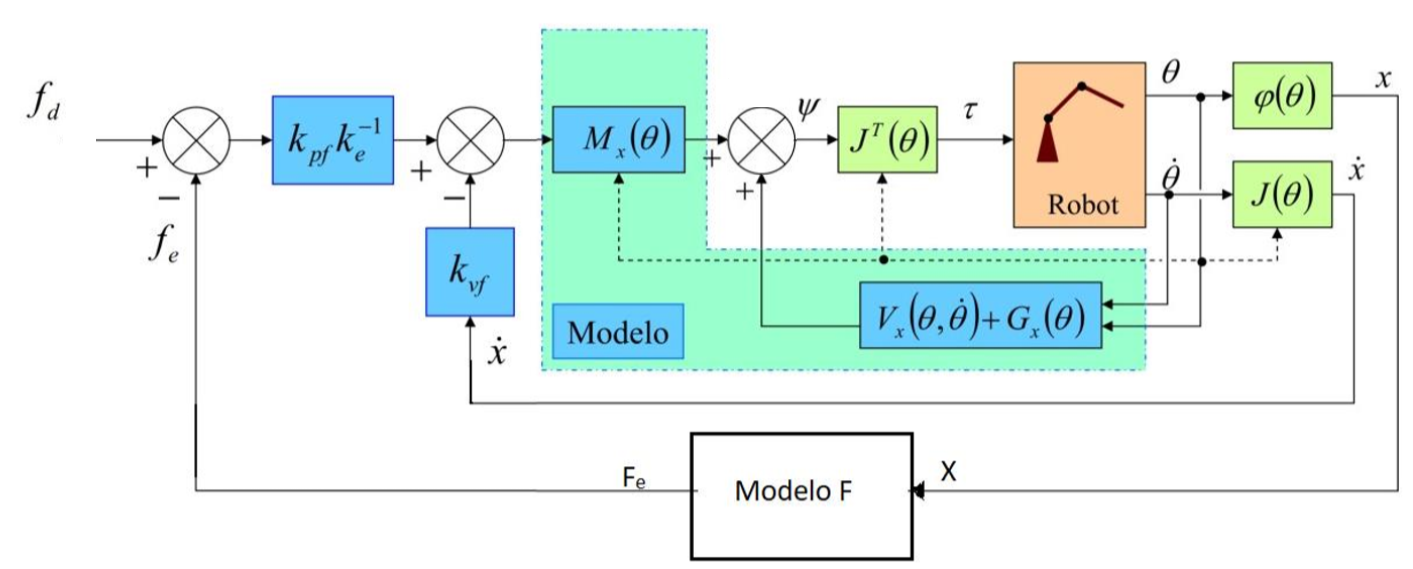
\includegraphics[width=0.8\linewidth]{ImagenesControl de fuerza no lineal/controlf}
	\caption{Topolog\'ia del control de fuerza no lineal.}	
	\label{fig:control_f_modelo}
\end{figure}


HABLAR DE VALROES DE GANANCIAS
\subsection{Resultados}
Se realiz\'o el simulink del sistema. Obteniendo los siguientes gr\'aficos.

\begin{figure}[H]
	\centering
	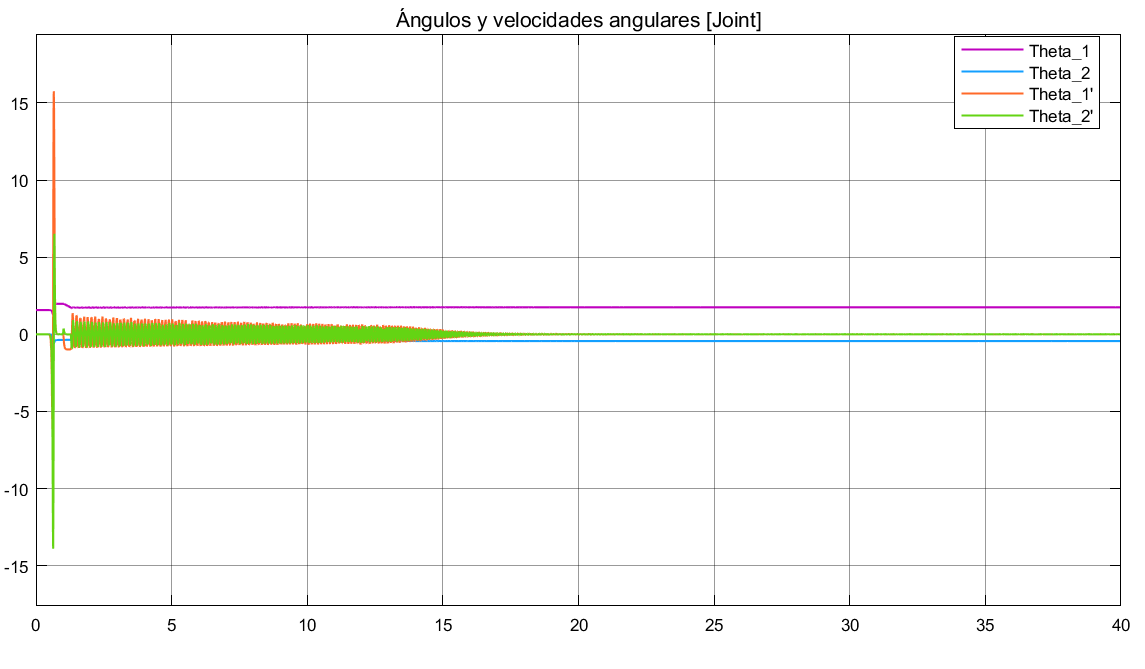
\includegraphics[width=0.8\linewidth]{ImagenesControl de fuerza no lineal/2_3_a}
	\caption{\'Angulos en funci\'on del tiempo en espacio joint.}	
	\label{fig:athetas}
\end{figure}

\begin{figure}[H]
	\centering
	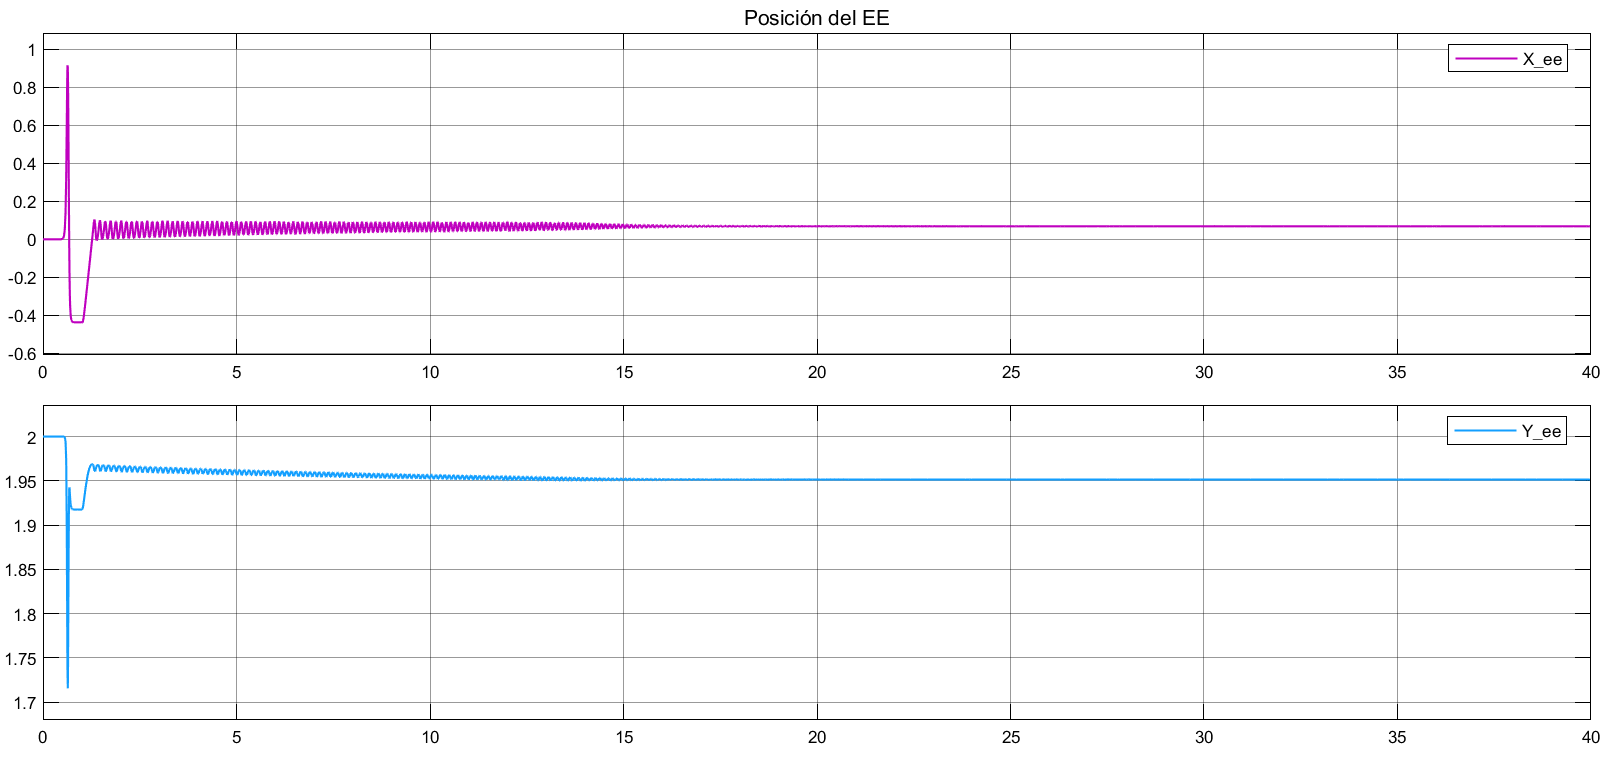
\includegraphics[width=0.8\linewidth]{ImagenesControl de fuerza no lineal/2_3_b}
	\caption{Posici\'on  del EE.}	
	\label{fig:apos}
\end{figure}
\begin{figure}[H]
	\centering
	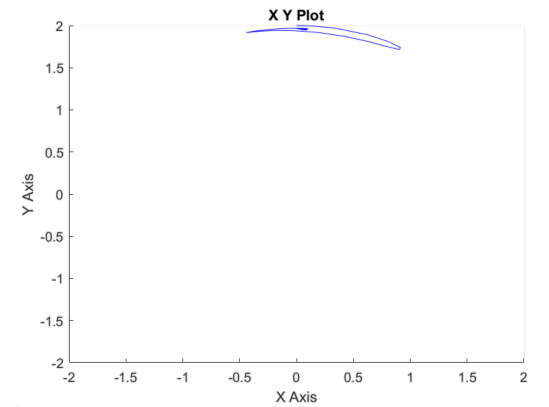
\includegraphics[width=0.5\linewidth]{ImagenesControl de fuerza no lineal/2_3_c}
	\caption{Gr\'afico XY.}	
	\label{fig:axy}
\end{figure}
\begin{figure}[H]
	\centering
	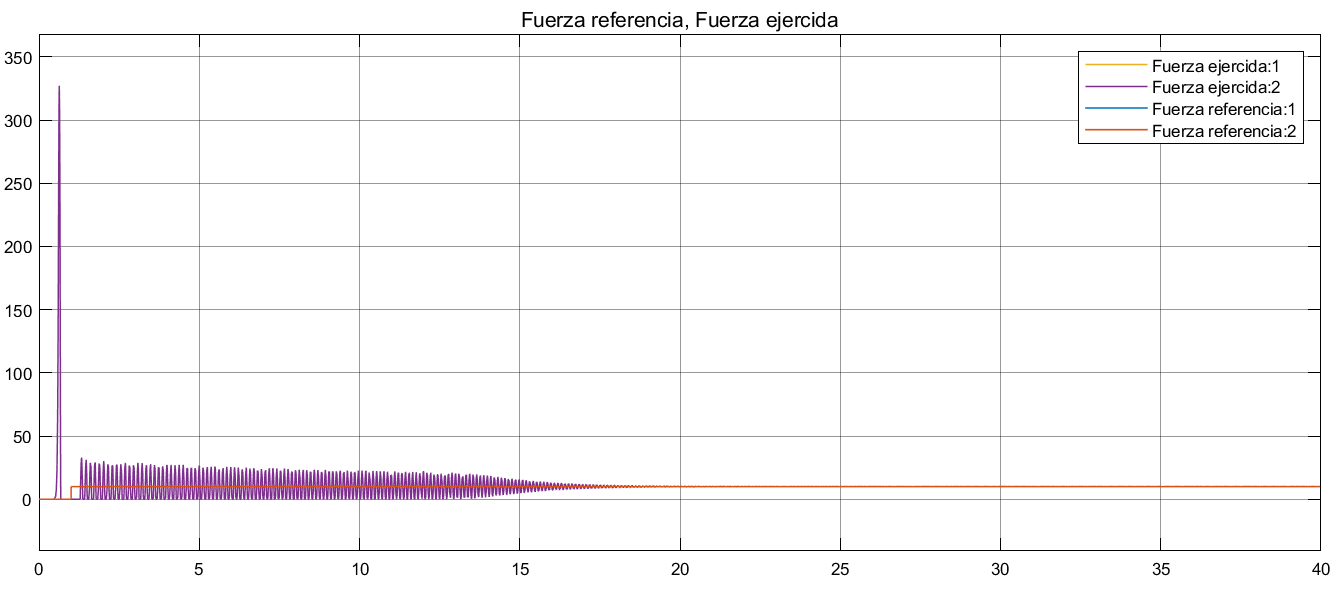
\includegraphics[width=0.8\linewidth]{ImagenesControl de fuerza no lineal/2_3_e}
	\caption{Gr\'afico XY.}	
	\label{fig:af}
\end{figure}
Ademas se le incluy\'o un disturbio a la planta tanto en posici\'on como en velocidad.
\begin{figure}[H]
	\centering
	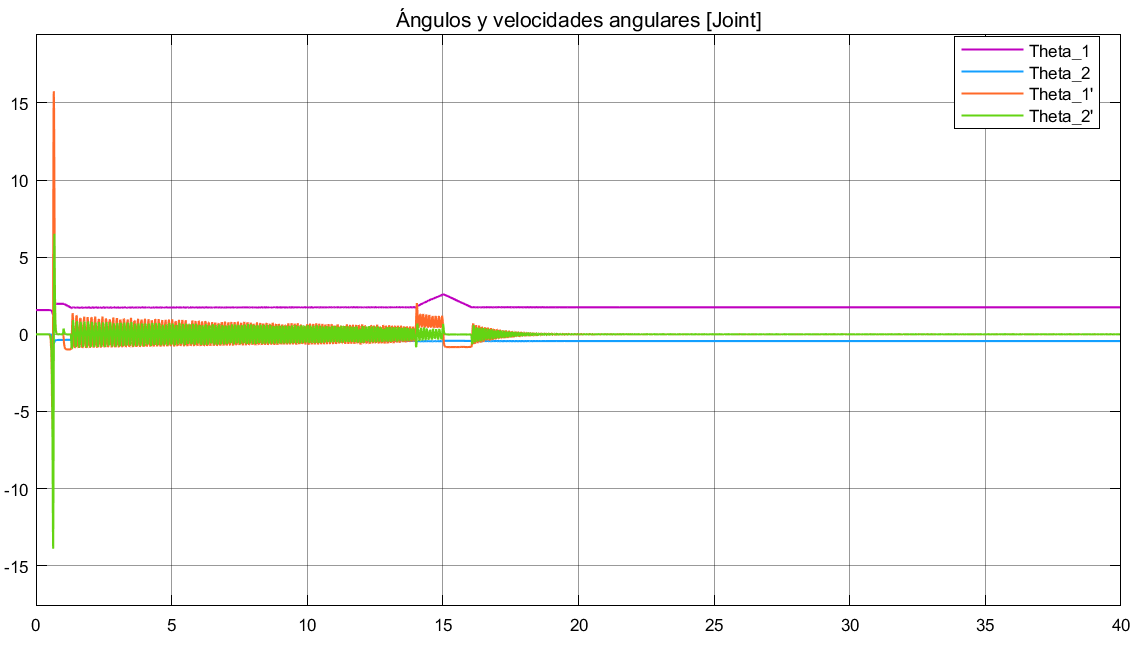
\includegraphics[width=0.8\linewidth]{ImagenesControl de fuerza no lineal/2_3_f_a}
	\caption{\'Angulos en funci\'on del tiempo en espacio joint.}	
	\label{fig:athetasd}
\end{figure}

\begin{figure}[H]
	\centering
	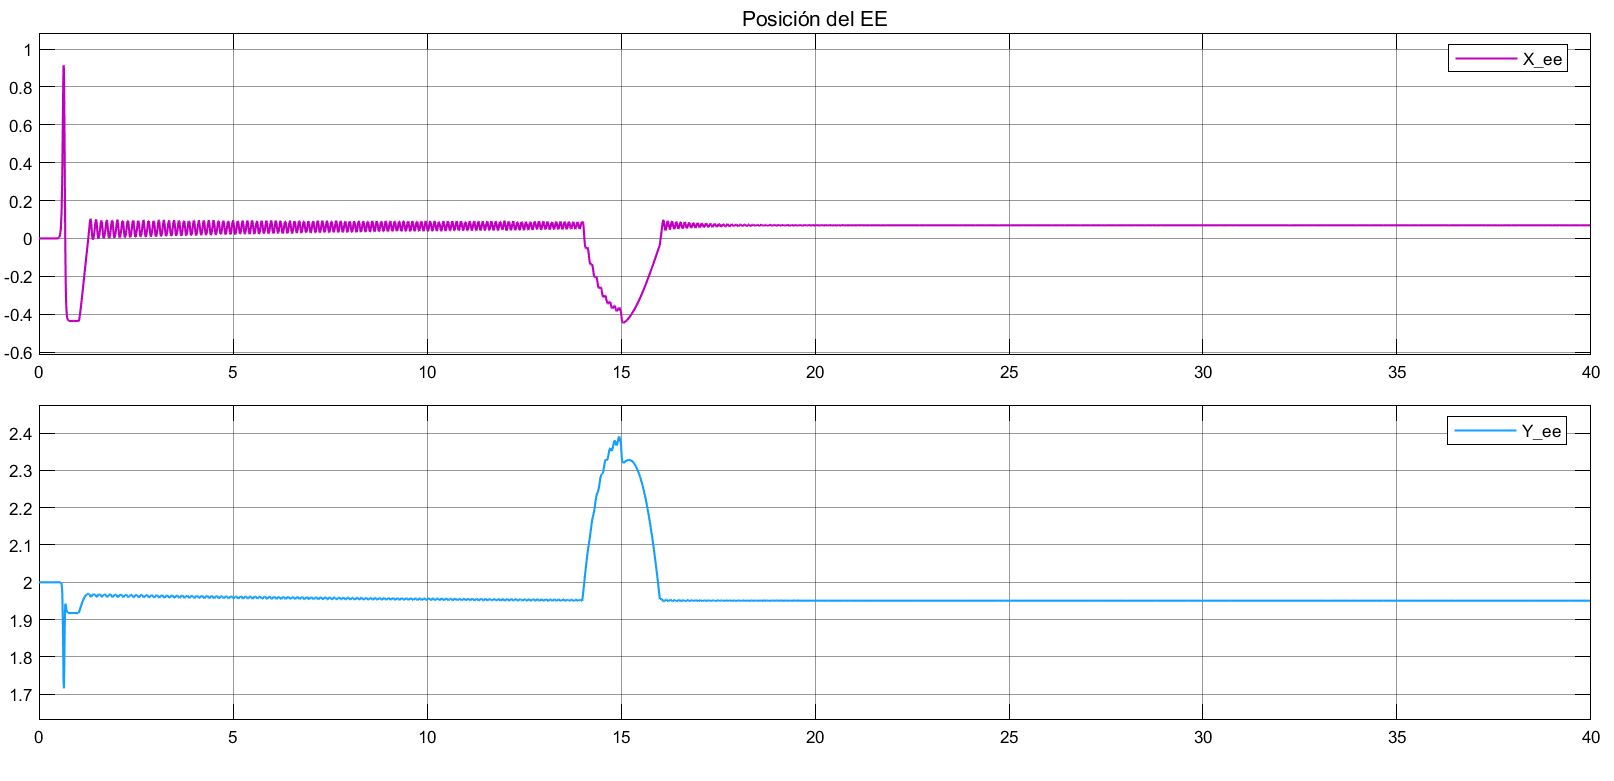
\includegraphics[width=0.8\linewidth]{ImagenesControl de fuerza no lineal/2_3_f_b}
	\caption{Posici\'on del EE.}	
	\label{fig:aposd}
\end{figure}
\begin{figure}[H]
	\centering
	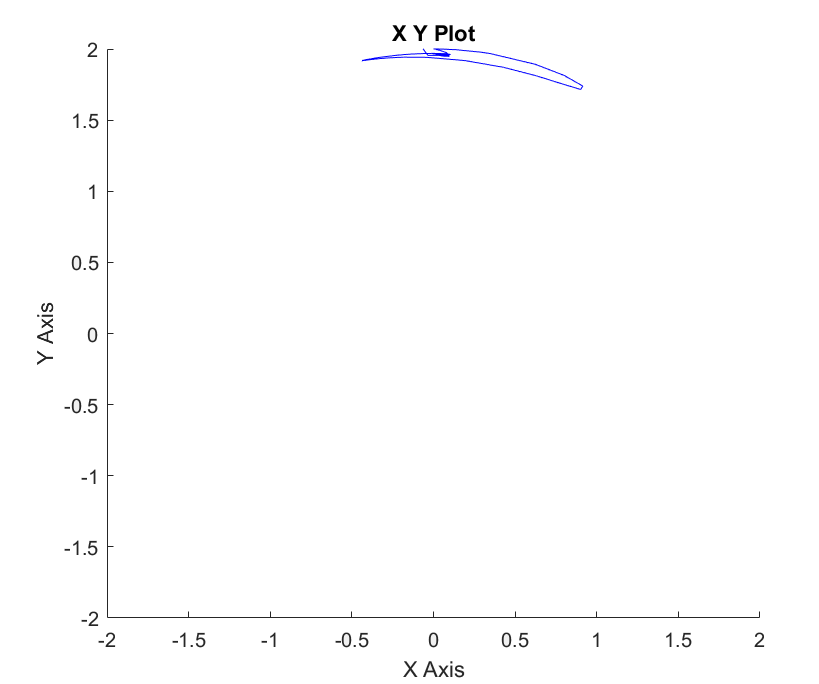
\includegraphics[width=0.5\linewidth]{ImagenesControl de fuerza no lineal/2_3_f_c}
	\caption{Gr\'afico XY.}	
	\label{fig:bxyd}
\end{figure}
\begin{figure}[H]
	\centering
	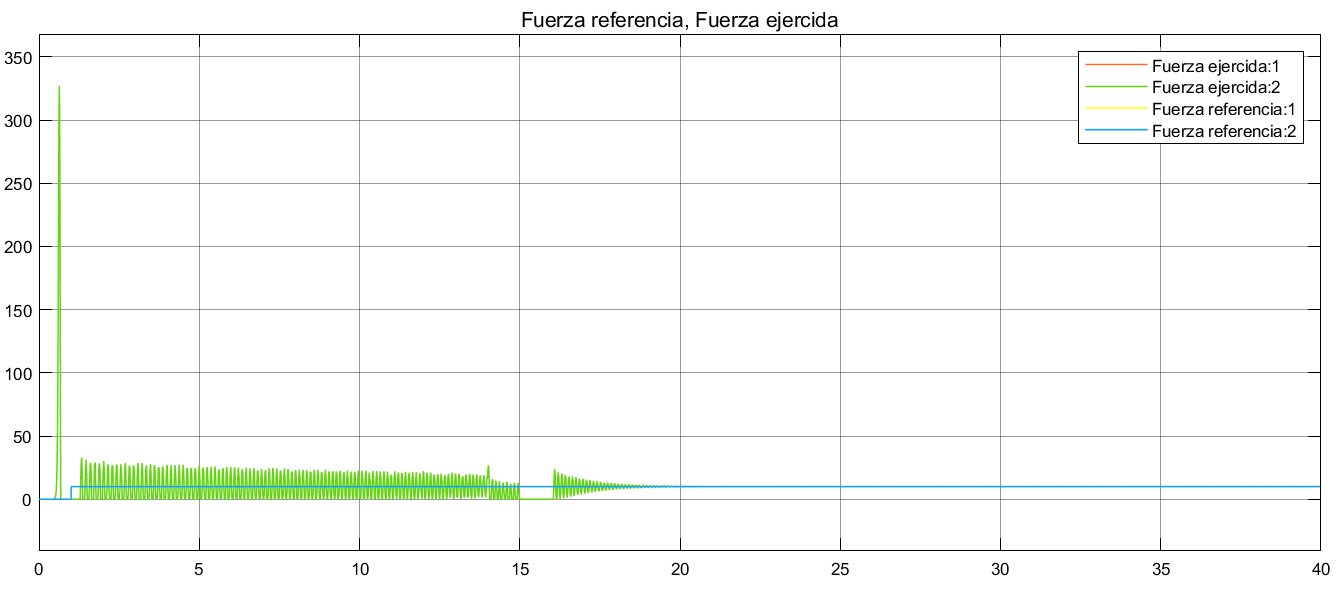
\includegraphics[width=0.8\linewidth]{ImagenesControl de fuerza no lineal/2_3_f_e}
	\caption{Fuerza deseada y real.}	
	\label{fig:bfd}
\end{figure}
%\end{document}
